\chapter{WebSocket-ak}

\index{WebSocket}WebSocket-ak jaio baino lehen, bezeroak zerbitzaritik datu bat jaso nahi zuenean, \index{AJAX}AJAX bidez egin behar zuen eskaera (\index{XmlHttpRequest}XmlHttpRequest edo \index{XHR}XHR objektu bat sortuz edo Fetch APIa erabiliz). Baliabide bakoitzeko XHR konexio bat ireki behar da: irudi bat lortzeko, JavaScript fitxategi bat atzitzeko, HTML orri bat jaisteko... 
Gauza bera bezeroak zerbitzarian dagoen prozesu baten egoera ezagutu nahiko balu:  une oro XHR eskaerak egin beharko lituzke (\textit{polling} delakoa\index{polling}). Prozedura hori ez da batere eraginkorra. Hoberena izango litzateke bezeroa entzuten jartzea eta zerbitzariak, noizbait bezeroari jakinarazi behar dion gertaeraren bat ikustean, bezeroari mezu bat bidaltzea. Hori da hain zuzen ere WebSocket APIaren zeregin nagusia. 

WebSocket-a ordenagailuen arteko \textit{full-duplex} edo bi norabideko komunikazioa lortzeko protokolo bat da, TCP konexio bakar baten gainean.

Horretaz aparte, nabarmendu daitekeen beste abantaila bat zera litzateke: WebSocket bat eraiki ondoren, bertatik bidaltzen diren pakete-goiburuen tamaina HTTP protokoloan erabiltzen direnena baino askoz txikiagoa da (ikus \ref{fig:wsheader}. irudia).


\begin{figure}[ht]
	\centering
\begin{tikzpicture}
\node[anchor=south west,inner sep=0] (image) at (0,0)
   {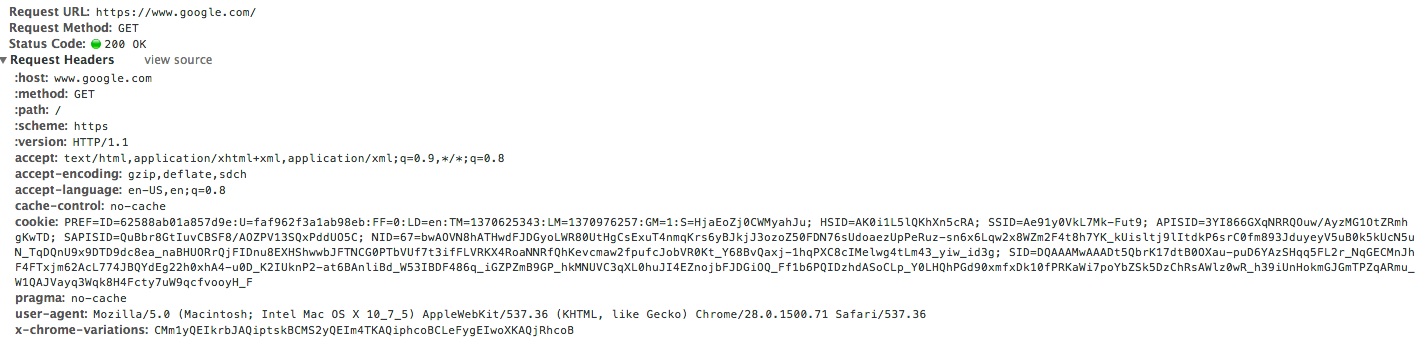
\includegraphics[trim=0cm 0cm 0cm 0cm, clip=true, width=1.0\textwidth]{img/http_header.png}};
\end{tikzpicture}
{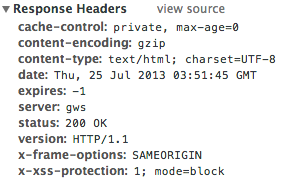
\includegraphics[trim=0cm 0cm 0cm 0cm, clip=true, width=0.5\textwidth]{img/ws_header.png}}
\caption{HTTPn pakete-goiburuen tamaina (goiko aldean, 1.356 byte) WebSocket protokoloan erabiltzen direnena (beheko aldean, 247 byte) baino askoz handiagoa da.}
\label{fig:wsheader}
\end{figure}


 WebSocket APIaz, HTTP zerbitzari baten kontra konexio bat ireki eta bertatik datuak jaso edo bidali ahal izango ditugu.  Zerbitzariak datu berriak bidali nahi dituenean, zuzenean egingo du, bezeroak ezer eskatu gabe. Horrez gain, WebSocket zerbitzari batek hainbat bezerorekin konexio irekiak izan ditzake aldi berean, bakoitzarekin \textit{socket} bat irekiz, komunikazioa denbora errealean garatuz. Gaur egun, HTML5en programatutako bideo-joko eta aldibereko talde-lana egiteko tresna askotan WebSocket-ak erabiltzen dira komunikazio eraginkorra lortzeko. Adibidez, Google Driven, dokumentu bat hainbat pertsonaren artean aldi berean editatzen dugunean, edo \ref{fig:whiteboard}. irudian ikusten dugun arbel digital partekatuan, WebSocket APIa erabiltzen ari gara.
 
 
\begin{figure}[ht]
	\centering
\begin{tikzpicture}
\node[anchor=south west,inner sep=0] (image) at (0,0)
   {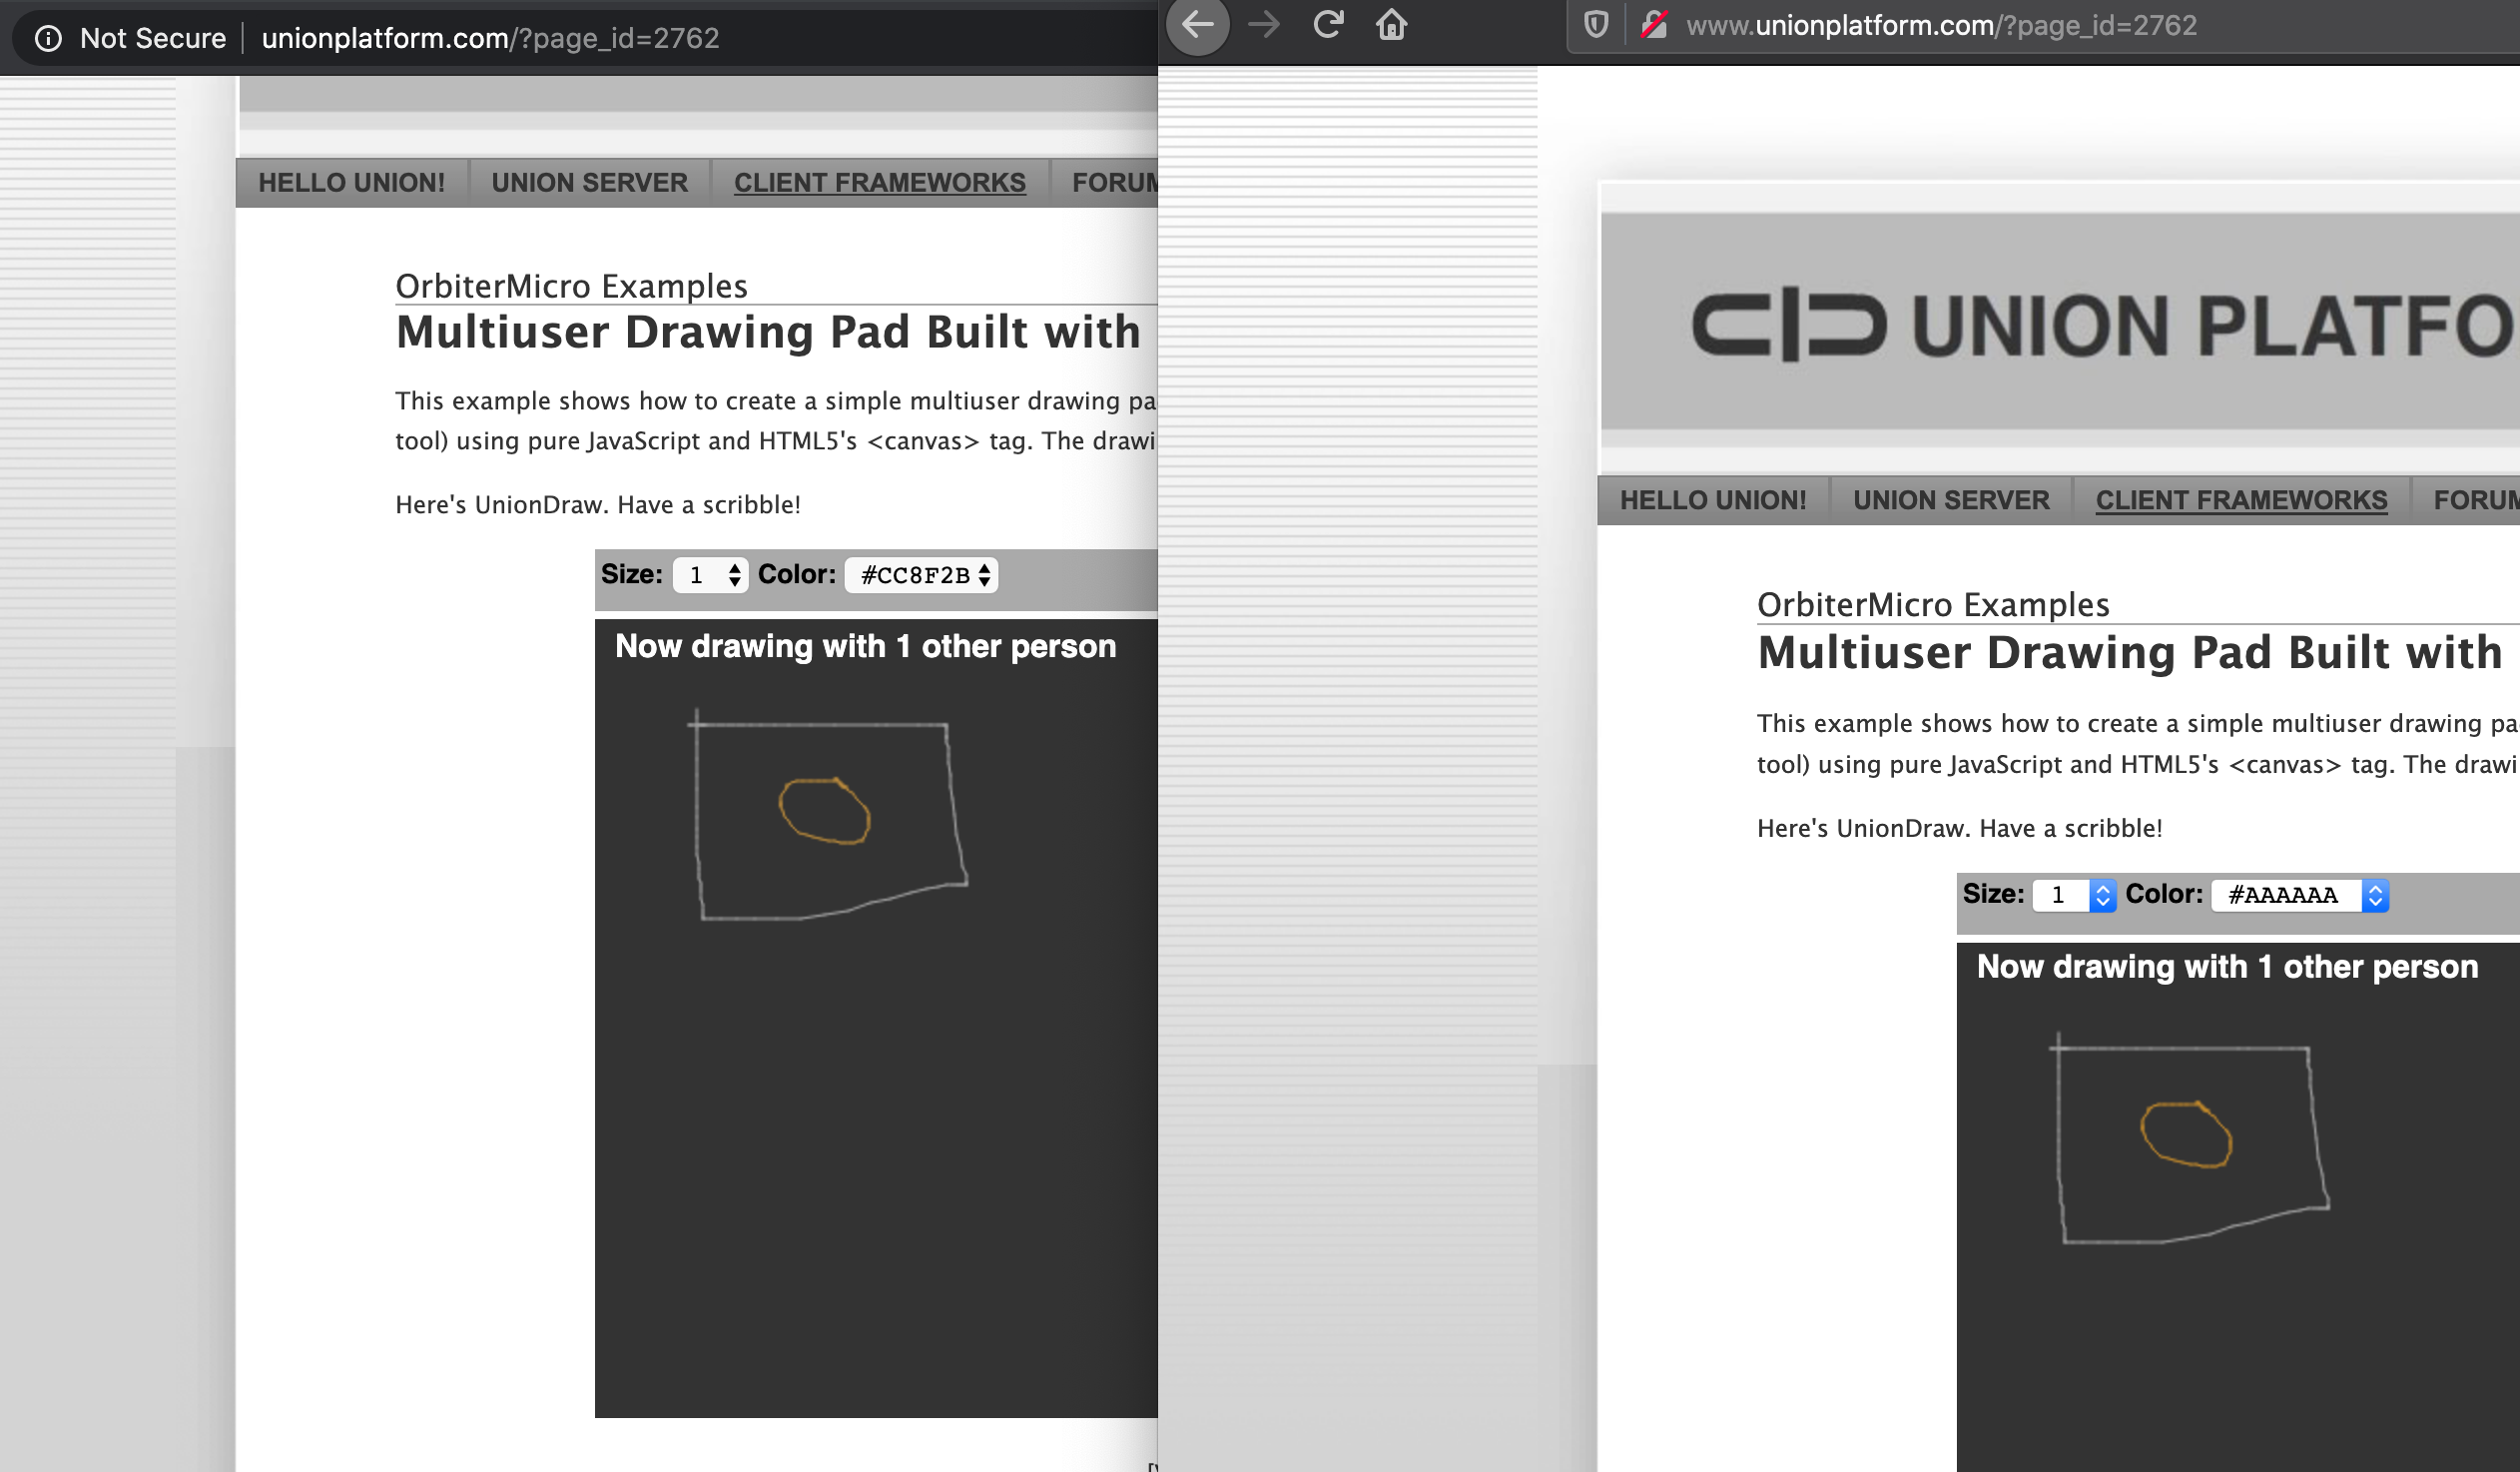
\includegraphics[trim=0cm 0cm 0cm 0cm, clip=true, width=1.0\textwidth]{img/whiteboardws.png}};
\end{tikzpicture}
\caption{WebSocket protokoloa erabiliz arbel digital partekatu bat programatu dezakegu, aldi berean hainbat erabiltzaileri bertan margotzeko aukera eskainiz. Iturria: \href{http://www.unionplatform.com/?page\_id=2762}{http://www.unionplatform.com/?page\_id=2762}.}
\label{fig:whiteboard}
\end{figure}


\section{WebSocket APIa nola erabili}

\subsection{Socket berri bat sortu (bezeroan)}

WebSocket-ek \index{ws}ws (edo \index{wss}wss, WebSocketSecure) protokoloa erabiliko dute HTTP edo HTTPS protokoloaren ordez.

Bezeroak socket-konexio berri bat sortu nahi duenean, WebSocket klasea instantziatuko du.

\begin{lstlisting}[language=JavaScript,numbers=none]
    let socket = new WebSocket("ws://domeinua/zerbitzua")
\end{lstlisting}

\subsection{Konexioa ezarri}

 Socketa irekitzean \textit{open} gertaera altxatuko da. Hori kudeatzeko \textit{socket.onopen} kudeatzailea zehaztuko dugu \index{onpen}:

 \begin{lstlisting}[language=JavaScript,numbers=none]
 socket.onopen = function(){
  console.log("Konexioa lortu da!");
}
\end{lstlisting}

\subsection{Mezuak jaso eta bidali}

Bezerotik zerbitzarira mezuak bidaltzeko \index{send}\textit{send} metodoaz baliatuko gara:

\begin{lstlisting}[language=JavaScript,numbers=none]
socket.send("mugimendu zuzena");
\end{lstlisting}

Bezeroak zerbitzaritik datozen mezuak entzuteko \index{onmessage}\textit{onmessage} izeneko \textit{callback} bat prestatuko du:

\begin{lstlisting}[language=JavaScript,numbers=none]

socket.onmessage = function(erantzuna) {
   console.log("Jasotako erantzuna: " + erantzuna.data);
}
\end{lstlisting}

Gaur egun ez da WebSocket APIa zuzenean programatzen, baizik eta horren ordez ospetsua egin den \index{socket.io}socket.io izeneko liburutegia erabiltzen da. Liburutegi hori bezeroan kargatzea erraza da:

\begin{lstlisting}[language=HTML,numbers=none]
    <script type="text/javascript" src="/socket.io/socket.io.js"></script>
\end{lstlisting}

Jabetu zaitez /socket.io/ karpetaren izena dela. Bertan dagoen \hl{socket.io.js}
fitxategiak gordetzen ditu erabil ditzakegun funtzioak, \textit{io} objektua barne. 

Hurrengo adibidean, \textit{socket.io} liburutegiaz baliatuko gara WebSocket konexio bat irekitzeko (\textit{connect} metodoaz). Jarraian \textit{socket}-etik mezuak bidaltzeko \index{emit}\textit{emit} metodoa erabiliko dugu.  Zerbitzaritik mezu bat jasotzean, \textit{socket.on} bidez zer funtzio egikarituko den zehazten da. Funtzioa jaso den mezuaren edukiaren arabera zehazten da. Adibidean, \hl{socket.on(\textquotesingle{}mugi\textquotesingle{})} dugu, baina baita \hl{socket.on(\textquotesingle{}phone-connect\textquotesingle{})} mezu mota ere. 

\begin{lstlisting}[language=JavaScript,numbers=none]
const serverURL = window.location.host;

// websocket zerbitzarira konektatu
export const socket = io.connect(serverURL);

// socket-atik mezu bat bidali
socket.emit('desktop-connect');

// socket-atik "mugi" mezu mota datorrenean
// mugitu metodoari deitu
socket.on('mugi', mugitu);

// socket-atik "phone-connect" mezu mota datorrenean
// phoneConnected metodoari deitu
socket.on('phone-connect', phoneConnected);

\end{lstlisting}

Zerbitzariaren aldetik, kodea oso antzekoa da.

\begin{lstlisting}[language=JavaScript,numbers=none]

const io = require('socket.io')(3000);

io.on('connection', socket => {
  // posible da mezu bat zuzenean bidaltzea
  socket.send('Hello!');

  // edo emit() bidez, gertaera zehatz batzuk bidaltzea
  socket.emit('mugi', {'nondik': 12, 'nora': 14});

  // bezeroak  socket.send() erabiliz gertaera bat bidali digu. Hori kudeatzeko:
  socket.on('message', (data) => {
    console.log(data);
  });

  // desktop-connect mezu mota jasotzean, kontsolan mezu bat bistaratuko dugu
  socket.on('desktop-connect', () => {
    console.log("Parametrorik gabeko deia");
  });
});

\end{lstlisting}

Zerbitzarian socket.io instalatzeko, \hl{npm} komando hau erabiliko dugu:
\begin{lstlisting}[language=Bash,numbers=none]
npm install socket.io
\end{lstlisting}

Oharra: npm, nodejs eta orokorrean zerbitzariaren aldeko kodearen inguruan beste liburu bat idatz daiteke. Nolanahi ere, honen inguruan oinarrizko ezagutza beharrezkoa ikusten denez, NodeJS-ri buruzko kapitulu bat eskaini da liburu honetan (ikus  \ref{chap:nodejs}. kapitulua).)

Zerbitzarian ez dugu soilik WebSocket bat izango, baizik eta hasierako HTTP protokoloa kudeatzeko zerbitzu bat ere eskaini behar dugu. Dena batera egin ahal izateko aurreko kodea apur bat aldatu beharra dago, honela:

\begin{lstlisting}[language=JavaScript,numbers=none]

const content = require('fs').readFileSync(__dirname + '/index.html', 'utf8');

const httpServer = require('http').createServer((req, res) => {
  // index.html orria zerbitzatu 
  res.setHeader('Content-Type', 'text/html');
  res.setHeader('Content-Length', Buffer.byteLength(content));
  res.end(content);
});

const io = require('socket.io')(httpServer);

io.on('connection', socket => {
  // posible da mezu bat zuzenean bidaltzea
  socket.send('Hello!');

  // edo emit() bidez, gertaera zehatz batzuk bidaltzea
  socket.emit('mugi', {"nondik": 12, "nora": 14});

  // bezeroak  socket.send() erabiliz gertaera bat bidali digu. Hori kudeatzeko:
  socket.on('desktop-connect', (data) => {
    console.log(data);
  });

});


httpServer.listen(3000, () => {
  console.log('go to http://localhost:3000');
});


\end{lstlisting}

Bezeroaren azken bertsioa, berriz, honela:

\begin{lstlisting}[language=HTML,numbers=none]
<!DOCTYPE html>
<html>
<head>
	<script type="text/javascript" src="/socket.io/socket.io.js"></script>
</head>

<body>

 <ul id="events"></ul>

	<script>
	
		// funtzio laguntzailea
		const $events = document.getElementById('events');
		const newItem = (content) => {
		  const item = document.createElement('li');
		  item.innerText = content;
		  return item;
		};


		// zerbitzariaren URLa
		const serverURL = window.location.host;
	
		console.log(serverURL);

		// websocket zerbitzarira konektatu
		const socket = io.connect(serverURL);

		// konexioa lortzean funtzio laguntzaileari deitu eta pantailan idatzi
		socket.on('connect', () => {
		console.log("Connect");
		  $events.appendChild(newItem('connect'));
		});

		// socket-atik mezu bat bidali
		socket.emit('desktop-connect', {"datuak": "adibide bat"});

		// socket-atik "mugi" edo "phone-connect" mezu mota datorrenean
		// newiItem metodoari deitu
		socket.on('mugi', (datuak) => {
					$events.appendChild(newItem(JSON.stringify( datuak)));
				});
	</script>


</body>
</html>
\end{lstlisting}

Adibidea probatzeko, terminal bat ireki eta, bertatik, \hlc[lightgray]{node server.js} komandoa landu.

Dena ondo badoa, http://localhost:3000 helbidean HTTP eta WS zerbitzaria entzuten egongo dira. Nabigatzailea irekitzean \ref{fig:websocketadibidea}. irudian ikusten dena ikusi beharko genuke. Bertan, dagoen lehenengo \textquotesingle{}connect\textquotesingle{} lerroa bezeroak zerbitzariaren kontra konexioa ondo irekitzean idatziko da. Hurrengo lerroa, berriz, zerbitzaritik \textquotesingle{}mugi\textquotesingle{} gertaera jasotzean agertuko da (gertaera horren barruan dauden datuak bistaratuz).

\begin{figure}[ht]
	\centering
\begin{tikzpicture}
\node[anchor=south west,inner sep=0] (image) at (0,0)
   {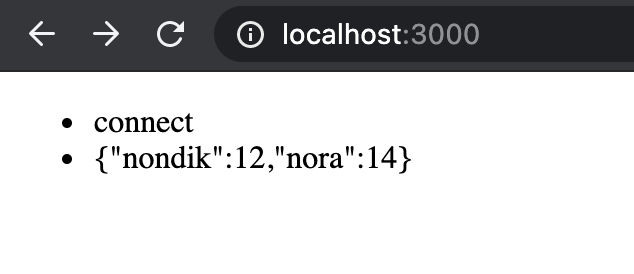
\includegraphics[trim=0cm 0cm 0cm 0cm, clip=true, width=.75\textwidth]{img/websockets/websocket.png}};
\end{tikzpicture}
\caption{WebSocket-en adibidea martxan jartzean horrelako emaitza lortu beharko genuke.}
\label{fig:websocketadibidea}
\end{figure}

Adibidearen kode osoa hemen aurkituko duzu:
\href{https://gist.github.com/juananpe/06df4742dae0cc01351089b5bed4c641}{https://labur.eus/5cEjB} (github.com).

\section{Ariketak}
WebSocket-ak eta mugikor bat erabiliko ditugu urruneko aginte bat programatzeko. Zehazki, pantailan grafiko bat bistaratuko da eta mugikorra eskuin aldera biratzean grafikoa eskuinera mugitu behar da. Ezkerrera biratzean, aldiz, grafikoa ezker aldera mugituko da (ikus \ref{fig:websocketariketa}. irudia).

\begin{figure}[ht]
	\centering
\begin{tikzpicture}
\node[anchor=south west,inner sep=0] (image) at (0,0)
   {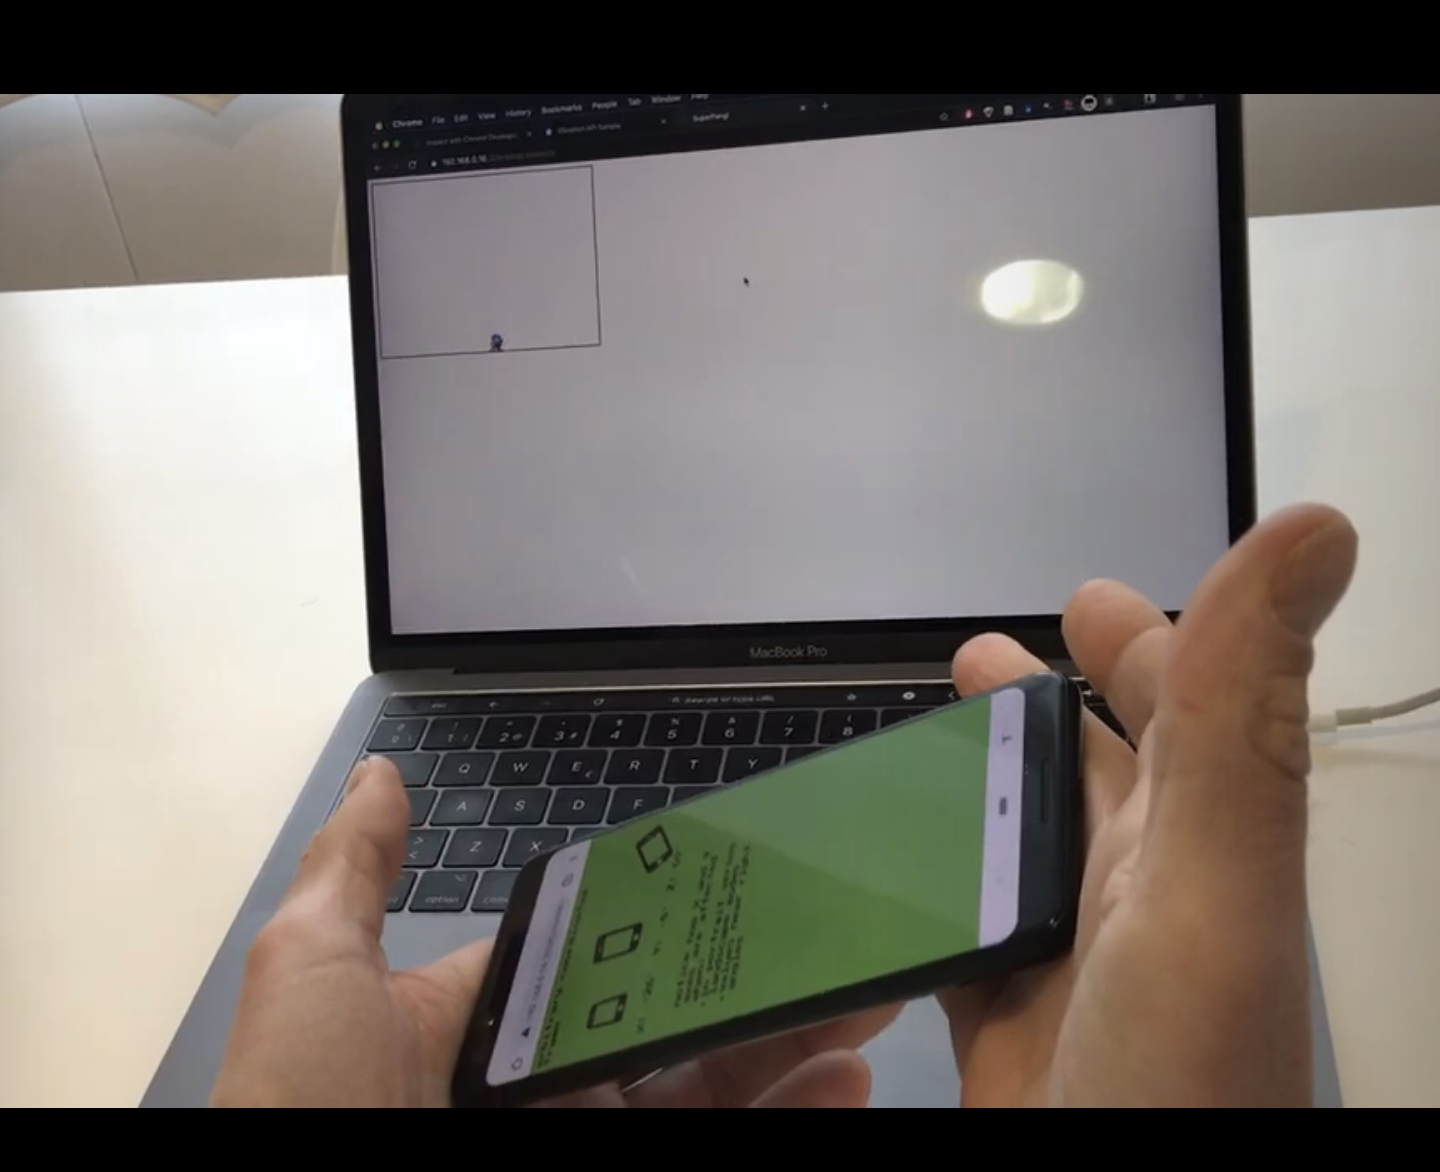
\includegraphics[trim=0cm 0cm 0cm 0cm, clip=true, width=1.0\textwidth]{img/websockets/websocketariketa.png}};
\end{tikzpicture}
\caption{WebSocket-ak erabiliz mugikor batetik kontrolatu dezakegu pantailan agertzen den irudi bat, ezker-eskuinera mugituz, mugikorra alde batera edo bestera biratzean.}
\label{fig:websocketariketa}
\end{figure}

Mugikorraren biraketak kontrolatzeko kodea hemen aurkituko duzu:\newline
\href{https://www.dropbox.com/s/dh81ca4f9isb44g/sockets\_mobile.zip?dl=1}{https://labur.eus/evkQ2} (dropbox.com).

Zerbitzariaren kode-txantiloia ere lagungarria aurkituko duzu: \href{https://gist.github.com/juananpe/6c27962e19163adb1bd145298d9ec611}{https://labur.eus/J9van} (github.com). NodeJS-n programatuta dago, beraz, ondo ulertzeko liburu honen NodeJS-ri buruzko gaia aztertzea gomendagarria da.